
\documentclass{article}

\usepackage{subcaption}
\usepackage{graphicx}
\usepackage{hyperref}

\title{ Livro dos antepassados }
\author{  }
\date{}

\begin{document}

\maketitle
\tableofcontents

\newpage
\newcounter{tablecounter}


\newpage
\section{Industrias reunidas 'Vilar'}


    
        \textit{by} Adelino Gonçalves Vilar
    


 
    \fbox{
        \begin{minipage}{0.9\textwidth}
            \vspace{0.2cm}
            \textbf{\textit{About}}
            \begin{itemize}
                
                    \item \textit{ José da Costa Vilar }
                
                    \item \textit{ Amadeu da Costa Vilar }
                
                    \item \textit{ Manuel da Costa Vilar }
                
            \end{itemize}
            \vspace{0.2cm}
        \end{minipage}
    }
    

    $\ast$~$\ast$~$\ast$  


    \begin{center}
        \begin{minipage}{0.9\textwidth}
            \setlength{\parskip}{0.2cm}
            \setlength{\parindent}{0cm}
            \fontsize{12pt}{14pt}\selectfont
            


Amigos e Srs:

Serve a presente para levar ao v/ conhecimento de que nesta data
trespachei as m/ indústrias de Moagem, Refrigerantes e Papel aos
m/filhos , José da Costa Vilar , Amadeu da Costa Vilar e Manuel da Costa Vilar, que, associando-se, continuarão a explorar as mesmas
indústrias.

Tomei esta decisão, porque o m/ precário estado de saúde assim o exigiu,
e fi-lo com satisfação por saber que os m/ filhos, que desde há muito
vinham colaborando comigo, são pessoas suficientemente competentes para
continuarem com os destinos das m/ indústrias.

Comunico também que fica todo o m/ Activo e Passivo ligado com as m/
indústrias até esta data a cargo da nova firma.

Ao abandonar esta carreira, quero agradecer a todos os m/ estimados
amigos, clientes e fornecedores todas as atenções com que sempre me
honraram e espero que continuarão a dispensar as mesmas aos m/
sucessores, que, certamente desempenharão por continuarem a bem servir
V. Exc.ª

Particularmente me ponho ao v/ dipor e tenho a honra de me subscrever
com a mais elevada estima e consideração.

De V. Excªs. M.to At.to Venr. e Obg.do

Adelino Gonçalves Vilar

        \end{minipage}
    \end{center}

    \stepcounter{tablecounter}
    
        \textsuperscript{\hyperref[table:\arabic{tablecounter}]{See metadata here}}
    


\newpage
\section{Industrias de Adelino Vilar}


    
        \textit{by} Manuel Vilar
    




    $\ast$~$\ast$~$\ast$  


    \begin{center}
        \begin{minipage}{0.9\textwidth}
            \setlength{\parskip}{0.2cm}
            \setlength{\parindent}{0cm}
            \fontsize{12pt}{14pt}\selectfont
            


Em Terroso, nas primeiras décadas do século, o meu pai, Adelino
Gonçalves Vilar, investiu em pequenas empresas, quase artesanais, dos
mais variados artigos, que na altura empregava alguns homens e
mulheresque não tinham outro modo de subsistência. Para ir substitutindo
os moinhos mais artesanai, fez uma fábrica de moagem, que com duas
pedras moía os cereais dos lavradores. No lugar do Vilar, onde residia
com a numerosa familia que constituiu, também teve uma pequena
fábrica/indústria de desnatar o leite das vacas para fazer a manteiga,
que era vendida em grandes caixas de madeira. Mais tarde montou uma
fábrica de refirgerntas que fabricava laranjadas, licores e também os
chamados 'pirolitos'. Além disso, criiou uma montagem de dois engenhos
para descascar linho e uma fábrica de fazer papel e cartir a partir da
reciclagem desses produtos, Para completar a lista recorde-se a
indústria de produzir tacões em madeira para calçado de homem e senhora.
Assim, em meados do século XX, Terroso foi talvez a freguesia com mais
empreendedorismo e indústrias do concelho da Póvoa de Varzim, no lugar
do Vilar, onde residia um Homem com o mesmo nome, e que foi o grande
responsável por essas obras dando, na altura grande nome à sua Terra e
ao seu desenvolvimento.

        \end{minipage}
    \end{center}

    \stepcounter{tablecounter}
    
        \textsuperscript{\hyperref[table:\arabic{tablecounter}]{See metadata here}}
    


\newpage
\section{Educação primária}


    
        \textit{by} Duarte Vilar
    


 
    \fbox{
        \begin{minipage}{0.9\textwidth}
            \vspace{0.2cm}
            \textbf{\textit{About}}
            \begin{itemize}
                
                    \item \textit{ avô Vilar }
                
                    \item \textit{ Vitalina }
                
            \end{itemize}
            \vspace{0.2cm}
        \end{minipage}
    }
    

    $\ast$~$\ast$~$\ast$  


    \begin{center}
        \begin{minipage}{0.9\textwidth}
            \setlength{\parskip}{0.2cm}
            \setlength{\parindent}{0cm}
            \fontsize{12pt}{14pt}\selectfont
            


Uma conversa muito engraçada, que acontece de forma recorrente entre o avô Vilar e sua esposa é sobre os seus "elevados graus de educação". Por norma
regista-se por alguma disputa ou conflito intelectual, e ultima com uma
das frases favoritas do meu avô ao dirigir-se à minha avó "Tu lá sabes
disso, só tens a 3ª classe..!". O meu avô só tem a 4ª.

        \end{minipage}
    \end{center}

    \stepcounter{tablecounter}
    
        \textsuperscript{\hyperref[table:\arabic{tablecounter}]{See metadata here}}
    


\newpage
\section{Pirolitos}


    
        \textit{by} ManuelVilar
    


 
    \fbox{
        \begin{minipage}{0.9\textwidth}
            \vspace{0.2cm}
            \textbf{\textit{About}}
            \begin{itemize}
                
                    \item \textit{ avô Vilar }
                
                    \item \textit{ Adelino Vilar }
                
                    \item \textit{ pirolitos }
                
            \end{itemize}
            \vspace{0.2cm}
        \end{minipage}
    }
    

    $\ast$~$\ast$~$\ast$  


    \begin{center}
        \begin{minipage}{0.9\textwidth}
            \setlength{\parskip}{0.2cm}
            \setlength{\parindent}{0cm}
            \fontsize{12pt}{14pt}\selectfont
            


A fábrica de refrigerantes Vilar foi construída pelo meu pai, Adelino Vilar, e por ele
herdada. As laranjadas e outro tipo de bebidas foram, durante muitos anos, distribuidas num
formato bastante peculiar. Hoje em dia utilizam-se especialmente
latas. Apesar de não tão longinquo, naquela época usavam-se garrafas de
vidro popularmente denominadas de pirolitos. Estas têm uma fisionomia
similar a qualquer outra garrafa de vidro, com a exceção do gargalo ter
em si imbutida uma bolinha de vidro solta. Qual o objetivo? Com a gasosa
a ser inserida na garrafa, a bolinha não tinha qualquer outra opção que
não ocupar o buraco do gargalo, selando a garrafa. As mesmas eram depois
recolhidas por funcionarios da empresa na rua, para as reutilizar. A
meio/parte final do governo de Salazar, estas garrafas foram abolidas
por supostos problemas de higiene.

        \end{minipage}
    \end{center}

    \stepcounter{tablecounter}
    
        \textsuperscript{\hyperref[table:\arabic{tablecounter}]{See metadata here}}
    


\newpage
\section{Viagem a cabo Verde}


    
        \textit{by} Duarte Manuel Vilar de Oliveira
    


 
    \fbox{
        \begin{minipage}{0.9\textwidth}
            \vspace{0.2cm}
            \textbf{\textit{About}}
            \begin{itemize}
                
                    \item \textit{ avô Vilar }
                
            \end{itemize}
            \vspace{0.2cm}
        \end{minipage}
    }
    

    $\ast$~$\ast$~$\ast$  


    \begin{center}
        \begin{minipage}{0.9\textwidth}
            \setlength{\parskip}{0.2cm}
            \setlength{\parindent}{0cm}
            \fontsize{12pt}{14pt}\selectfont
            


Após uma visita ao meu irmão a Lisboa naquela que foi uma estadia de
pouco menos de uma semana regressamos juntos a casa, na Póvoa, e
decidimos visitar os nossos avós maternos com os quais já não estávamos
há umas semanas.

Depois dos usuais cumprimentos e saudações entre avós e netos
sentamo-nos a conversar sobre a nossa vida, acompanhados de alguns
comentários sobre a atualidade política e social. A meio do diálogo o
meu irmão informa meus avós que vai partir para Cabo Verde na semana que
se avizinha. Apesar de contente, o meu lamenta-se profundamente, dizendo
que apesar de já ter *visitado meio mundo* *Egito, Jerusalém, quase toda
a Europa e também o Brasil* ainda não tinha conhecido essa ilha *outrora
pertencente a Portugal*. Num impulso, diz que *há de falar com a nossa
madrinha para ver umas viagens* e que um dia também irá também calcar
solo cabo-verdense, ao mesmo tempo que a minha revira os olhos em
discórdia e desacreditar. Rimo-nos.

        \end{minipage}
    \end{center}

    \stepcounter{tablecounter}
    
        \textsuperscript{\hyperref[table:\arabic{tablecounter}]{See metadata here}}
    


\newpage
\section{Prenda de Natal 2004}


    
        \textit{by} Duarte Manuel Vilar de Oliveira
    


 
    \fbox{
        \begin{minipage}{0.9\textwidth}
            \vspace{0.2cm}
            \textbf{\textit{About}}
            \begin{itemize}
                
                    \item \textit{ rádio Onda Viva }
                
                    \item \textit{ avô Vilar }
                
            \end{itemize}
            \vspace{0.2cm}
        \end{minipage}
    }
    

    $\ast$~$\ast$~$\ast$  


    \begin{center}
        \begin{minipage}{0.9\textwidth}
            \setlength{\parskip}{0.2cm}
            \setlength{\parindent}{0cm}
            \fontsize{12pt}{14pt}\selectfont
            


Tinha eu cerca de 4 anos (talvez fossem 3, mas sem grandes certezas), na
altura ainda andava no infantário, e umas 2 semanas antes do Natal, já
em ambiente natalício veio a rádio Onda Viva entrevistar os alunos desse
infantário. Queriam saber o que nós gostavamos de receber pelo Natal.
Sendo eu sempre irreverente e sem vergonha, mal o microfone chegou à
minha face, gritei que era o Duarte e que o que queria no Natal era uma
moto 4.

Aqui entre nós, nem sei bem o que me passou pela cabeça para
dizer aquilo, mas a verdade é que nesse mesmo momento estava o meu avô
Vilar a ir para o Porto, de carro, com o rádio sintonizado na rádio Onda
Viva. Coincidências das coincidências, até porque ele costuma ouvir a
rádio Renascença, ouviu o meu pedido e para além de uma risota geral na
minha família quando lhes contou, sempre recebi uma enorme moto 4 nesse
mesmo Natal, daquelas que dá para conduzir e tudo.

        \end{minipage}
    \end{center}

    \stepcounter{tablecounter}
    
        \textsuperscript{\hyperref[table:\arabic{tablecounter}]{See metadata here}}
    


\newpage
\section{Roupa a secar}


    
        \textit{by} False
    


 
    \fbox{
        \begin{minipage}{0.9\textwidth}
            \vspace{0.2cm}
            \textbf{\textit{About}}
            \begin{itemize}
                
                    \item \textit{ avô Vilar }
                
            \end{itemize}
            \vspace{0.2cm}
        \end{minipage}
    }
    

    $\ast$~$\ast$~$\ast$  


    \begin{center}
        \begin{minipage}{0.9\textwidth}
            \setlength{\parskip}{0.2cm}
            \setlength{\parindent}{0cm}
            \fontsize{12pt}{14pt}\selectfont
            


Falava-se, antigamente, de algumas coisas associadas a dias especiais.
Mau olhado e coisas do género. As pessoas geriam-se muito pelo que se
falava e o "diabo estava sempre à espreita". Uma das coisas que não se
fazia na nossa casa era pôr roupa a secar no dia da passagem de ano.
Dizia-se que dava azar.

(Escusado será dizer que o meu avô ria-se destes cuidados da minha avó. Não
faziam sentido, dizia ele.)

        \end{minipage}
    \end{center}

    \stepcounter{tablecounter}
    
        \textsuperscript{\hyperref[table:\arabic{tablecounter}]{See metadata here}}
    


\newpage
\section{Pobreza}


    
        \textit{by} Vitalina Moreira Martins
    


 
    \fbox{
        \begin{minipage}{0.9\textwidth}
            \vspace{0.2cm}
            \textbf{\textit{About}}
            \begin{itemize}
                
                    \item \textit{ açaipas }
                
                    \item \textit{ sulipas }
                
            \end{itemize}
            \vspace{0.2cm}
        \end{minipage}
    }
    

    $\ast$~$\ast$~$\ast$  


    \begin{center}
        \begin{minipage}{0.9\textwidth}
            \setlength{\parskip}{0.2cm}
            \setlength{\parindent}{0cm}
            \fontsize{12pt}{14pt}\selectfont
            


Senti talvez que fosse proveitoso acoplar um conjunto de pequenas
histórias da minha avó relativamente à pobreza que a rodeava, na sua
infância e juventude.

Um problema que havia nos campos, e que afligia principalmente aqueles
que eram mais descuidados e deixavam material para a labuta no campo
durante a noite, ou nalgum sitio mais exposto era que pela miséria,
muitos roubavam as de couro que eram usadas no gado para fazer um tipo de chinelos. As
sulipas, segundo ela, eram basicamente umas solas de couro que se
prendiam ao pé, para aqueles que não tinham dinheiro sequer para
calçado.

        \end{minipage}
    \end{center}

    \stepcounter{tablecounter}
    
        \textsuperscript{\hyperref[table:\arabic{tablecounter}]{See metadata here}}
    



\clearpage
\section{Images}

\newcounter{image}



    \begin{figure}[ht!]
        \begin{minipage}{0.35\textwidth}
            \centering
            \includegraphics[width=\linewidth]{/mnt/c/Users/Duarte Vilar/OneDrive/Ambiente de Trabalho/Eu/tese/thesis/Thesis/Vilar/AdelinoVilar/p1-Adelino.jpg}
            \caption{a future caption here}
        \end{minipage}
        \hspace{1cm} % add some horizontal space here
        \begin{minipage}{0.3\textwidth}
            ok

            palavra 2

            palavra 3

            lasjgslakgjalkjgsalkj

            arroz
            
        \end{minipage}
    \end{figure}



    \begin{figure}[ht!]
        \begin{minipage}{0.35\textwidth}
            \centering
            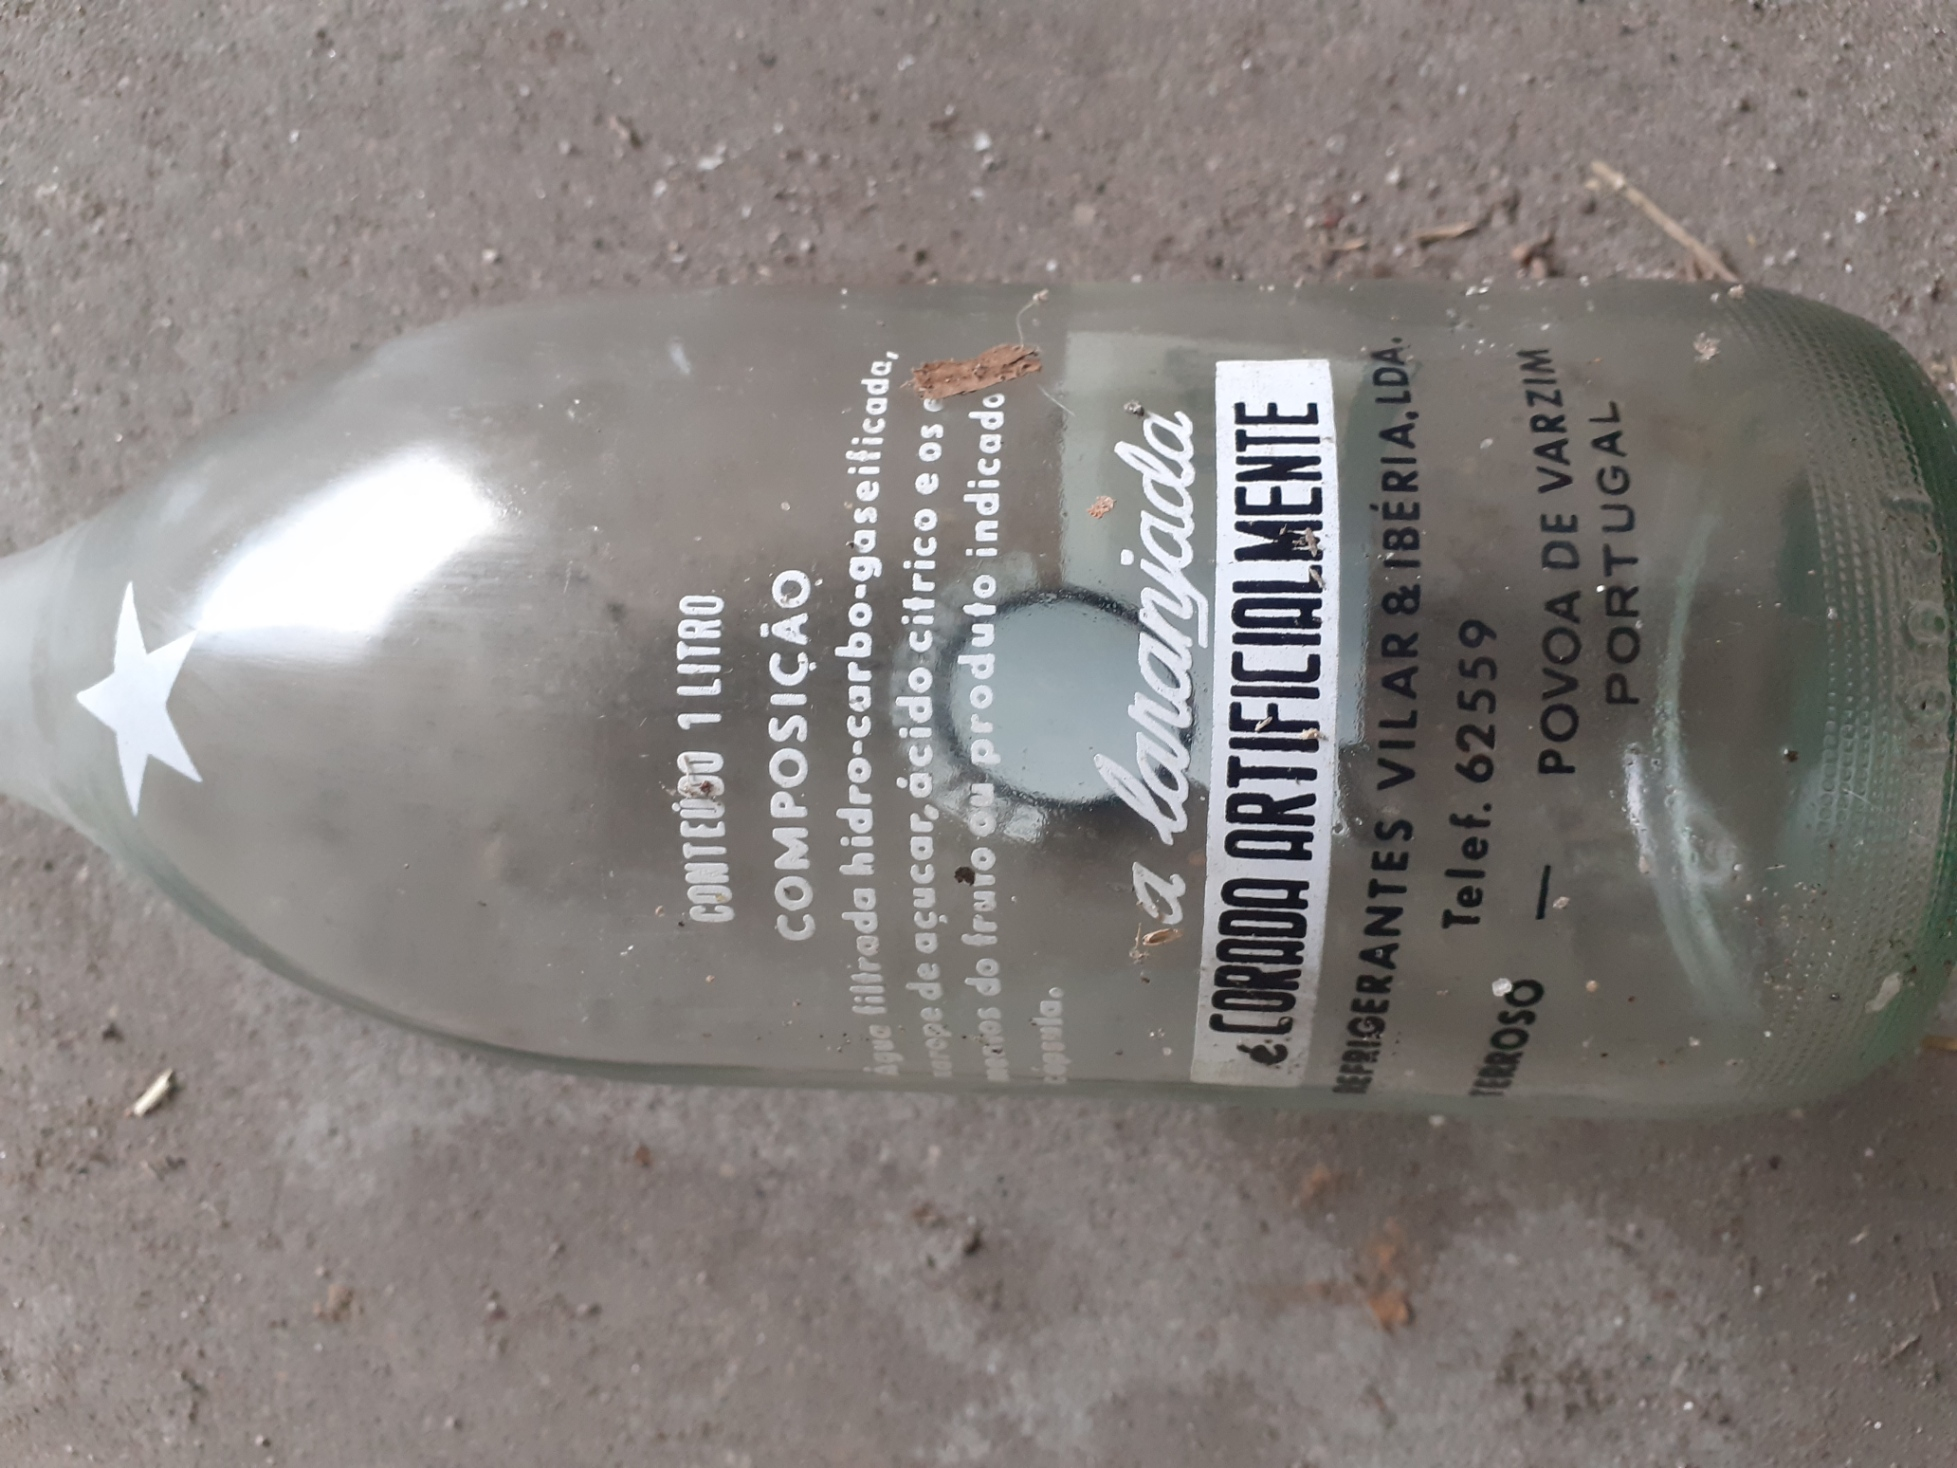
\includegraphics[width=\linewidth]{/mnt/c/Users/Duarte Vilar/OneDrive/Ambiente de Trabalho/Eu/tese/thesis/Thesis/Vilar/AdelinoVilar/p2-laranjada.jpg}
            \caption{a future caption here}
        \end{minipage}
        \hspace{1cm} % add some horizontal space here
        \begin{minipage}{0.3\textwidth}
            ok

            palavra 2

            palavra 3

            lasjgslakgjalkjgsalkj

            arroz
            
        \end{minipage}
    \end{figure}



    \begin{figure}[ht!]
        \begin{minipage}{0.35\textwidth}
            \centering
            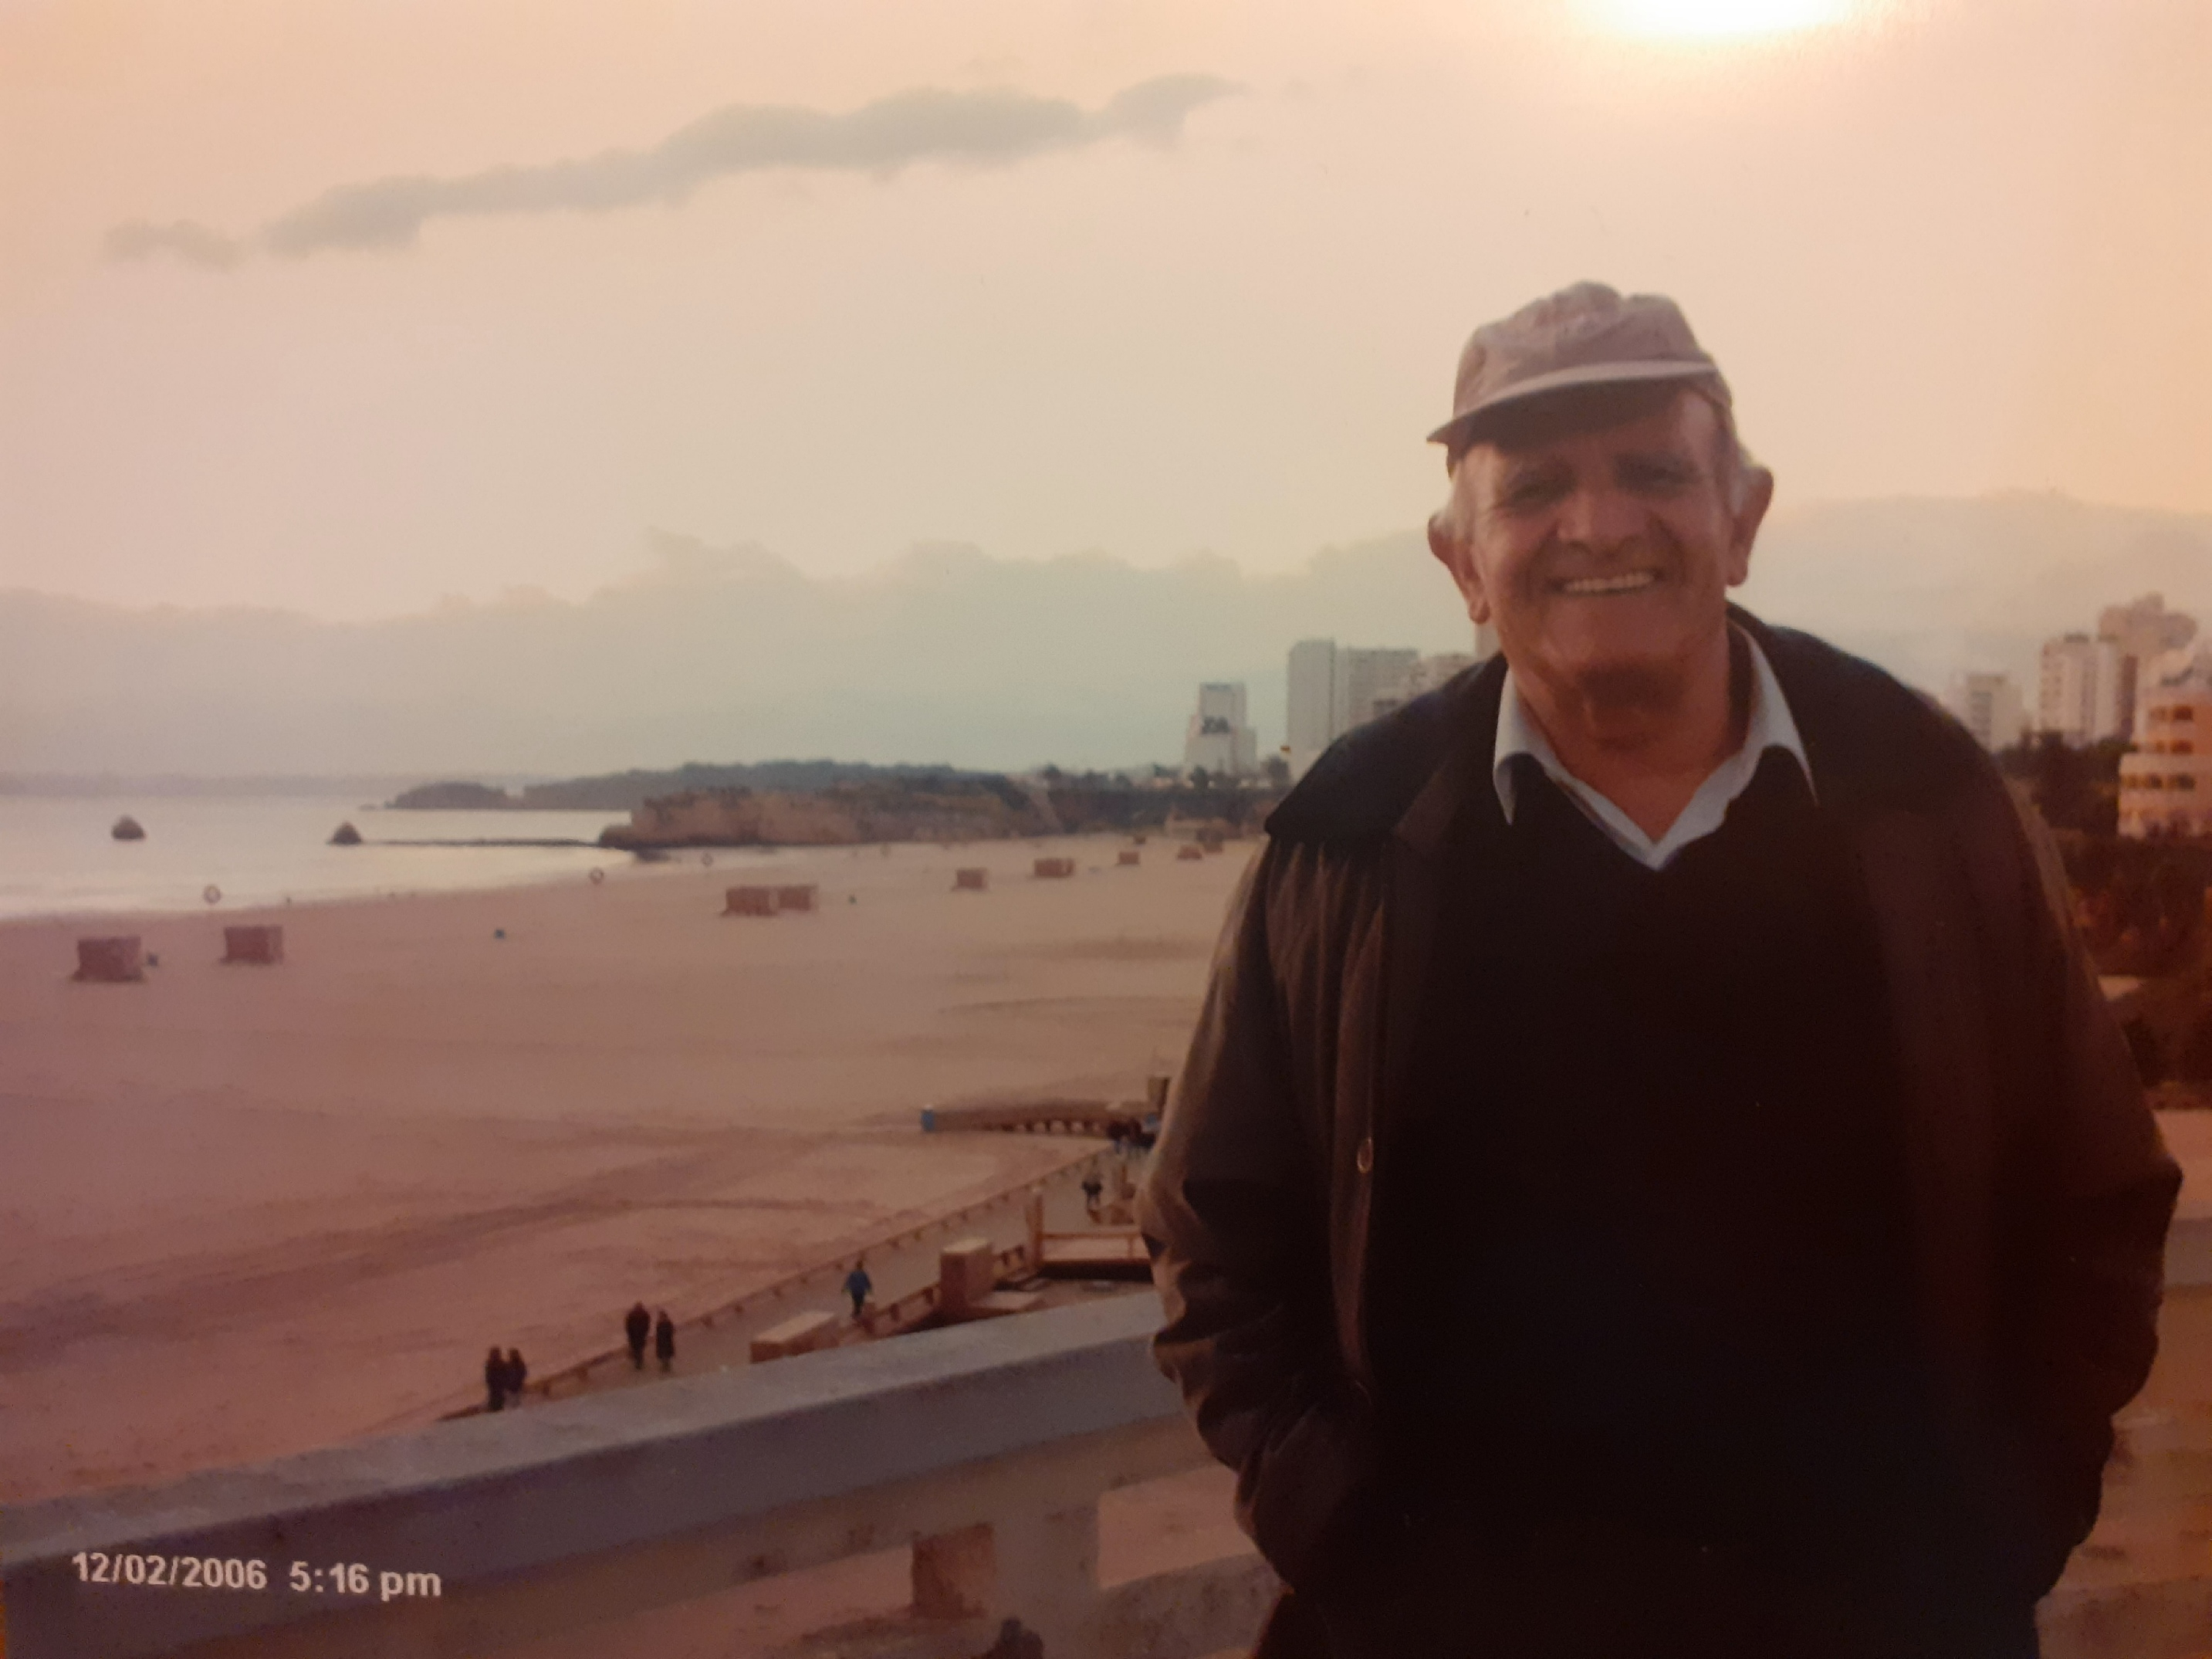
\includegraphics[width=\linewidth]{/mnt/c/Users/Duarte Vilar/OneDrive/Ambiente de Trabalho/Eu/tese/thesis/Thesis/Vilar/AdelinoVilar/ManuelVilar/p5-avoVilar.jpg}
            \caption{a future caption here}
        \end{minipage}
        \hspace{1cm} % add some horizontal space here
        \begin{minipage}{0.3\textwidth}
            ok

            palavra 2

            palavra 3

            lasjgslakgjalkjgsalkj

            arroz
            
        \end{minipage}
    \end{figure}



    \begin{figure}[ht!]
        \begin{minipage}{0.35\textwidth}
            \centering
            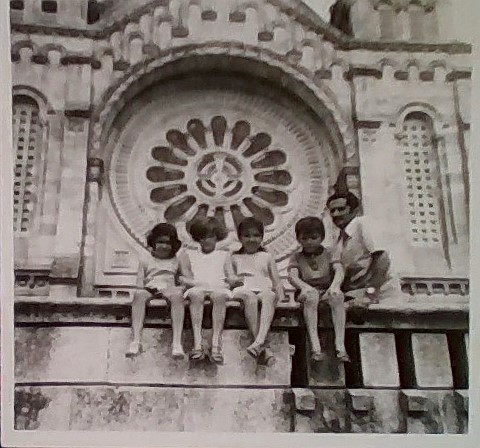
\includegraphics[width=\linewidth]{/mnt/c/Users/Duarte Vilar/OneDrive/Ambiente de Trabalho/Eu/tese/thesis/Thesis/Vilar/AdelinoVilar/ManuelVilar/ClaraVilar/p2-tioAntonio.jpg}
            \caption{a future caption here}
        \end{minipage}
        \hspace{1cm} % add some horizontal space here
        \begin{minipage}{0.3\textwidth}
            ok

            palavra 2

            palavra 3

            lasjgslakgjalkjgsalkj

            arroz
            
        \end{minipage}
    \end{figure}



    \begin{figure}[ht!]
        \begin{minipage}{0.35\textwidth}
            \centering
            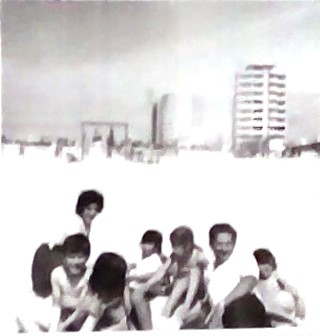
\includegraphics[width=\linewidth]{/mnt/c/Users/Duarte Vilar/OneDrive/Ambiente de Trabalho/Eu/tese/thesis/Thesis/Vilar/AdelinoVilar/ManuelVilar/ClaraVilar/p3-praiaTioAntonio.jpg}
            \caption{a future caption here}
        \end{minipage}
        \hspace{1cm} % add some horizontal space here
        \begin{minipage}{0.3\textwidth}
            ok

            palavra 2

            palavra 3

            lasjgslakgjalkjgsalkj

            arroz
            
        \end{minipage}
    \end{figure}



    \begin{figure}[ht!]
        \begin{minipage}{0.35\textwidth}
            \centering
            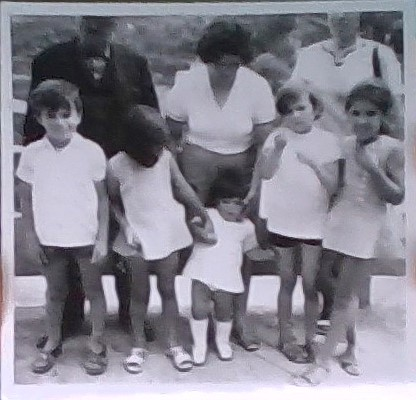
\includegraphics[width=\linewidth]{/mnt/c/Users/Duarte Vilar/OneDrive/Ambiente de Trabalho/Eu/tese/thesis/Thesis/Vilar/AdelinoVilar/ManuelVilar/ClaraVilar/p4-primosClara.jpg}
            \caption{a future caption here}
        \end{minipage}
        \hspace{1cm} % add some horizontal space here
        \begin{minipage}{0.3\textwidth}
            ok

            palavra 2

            palavra 3

            lasjgslakgjalkjgsalkj

            arroz
            
        \end{minipage}
    \end{figure}



    \begin{figure}[ht!]
        \begin{minipage}{0.35\textwidth}
            \centering
            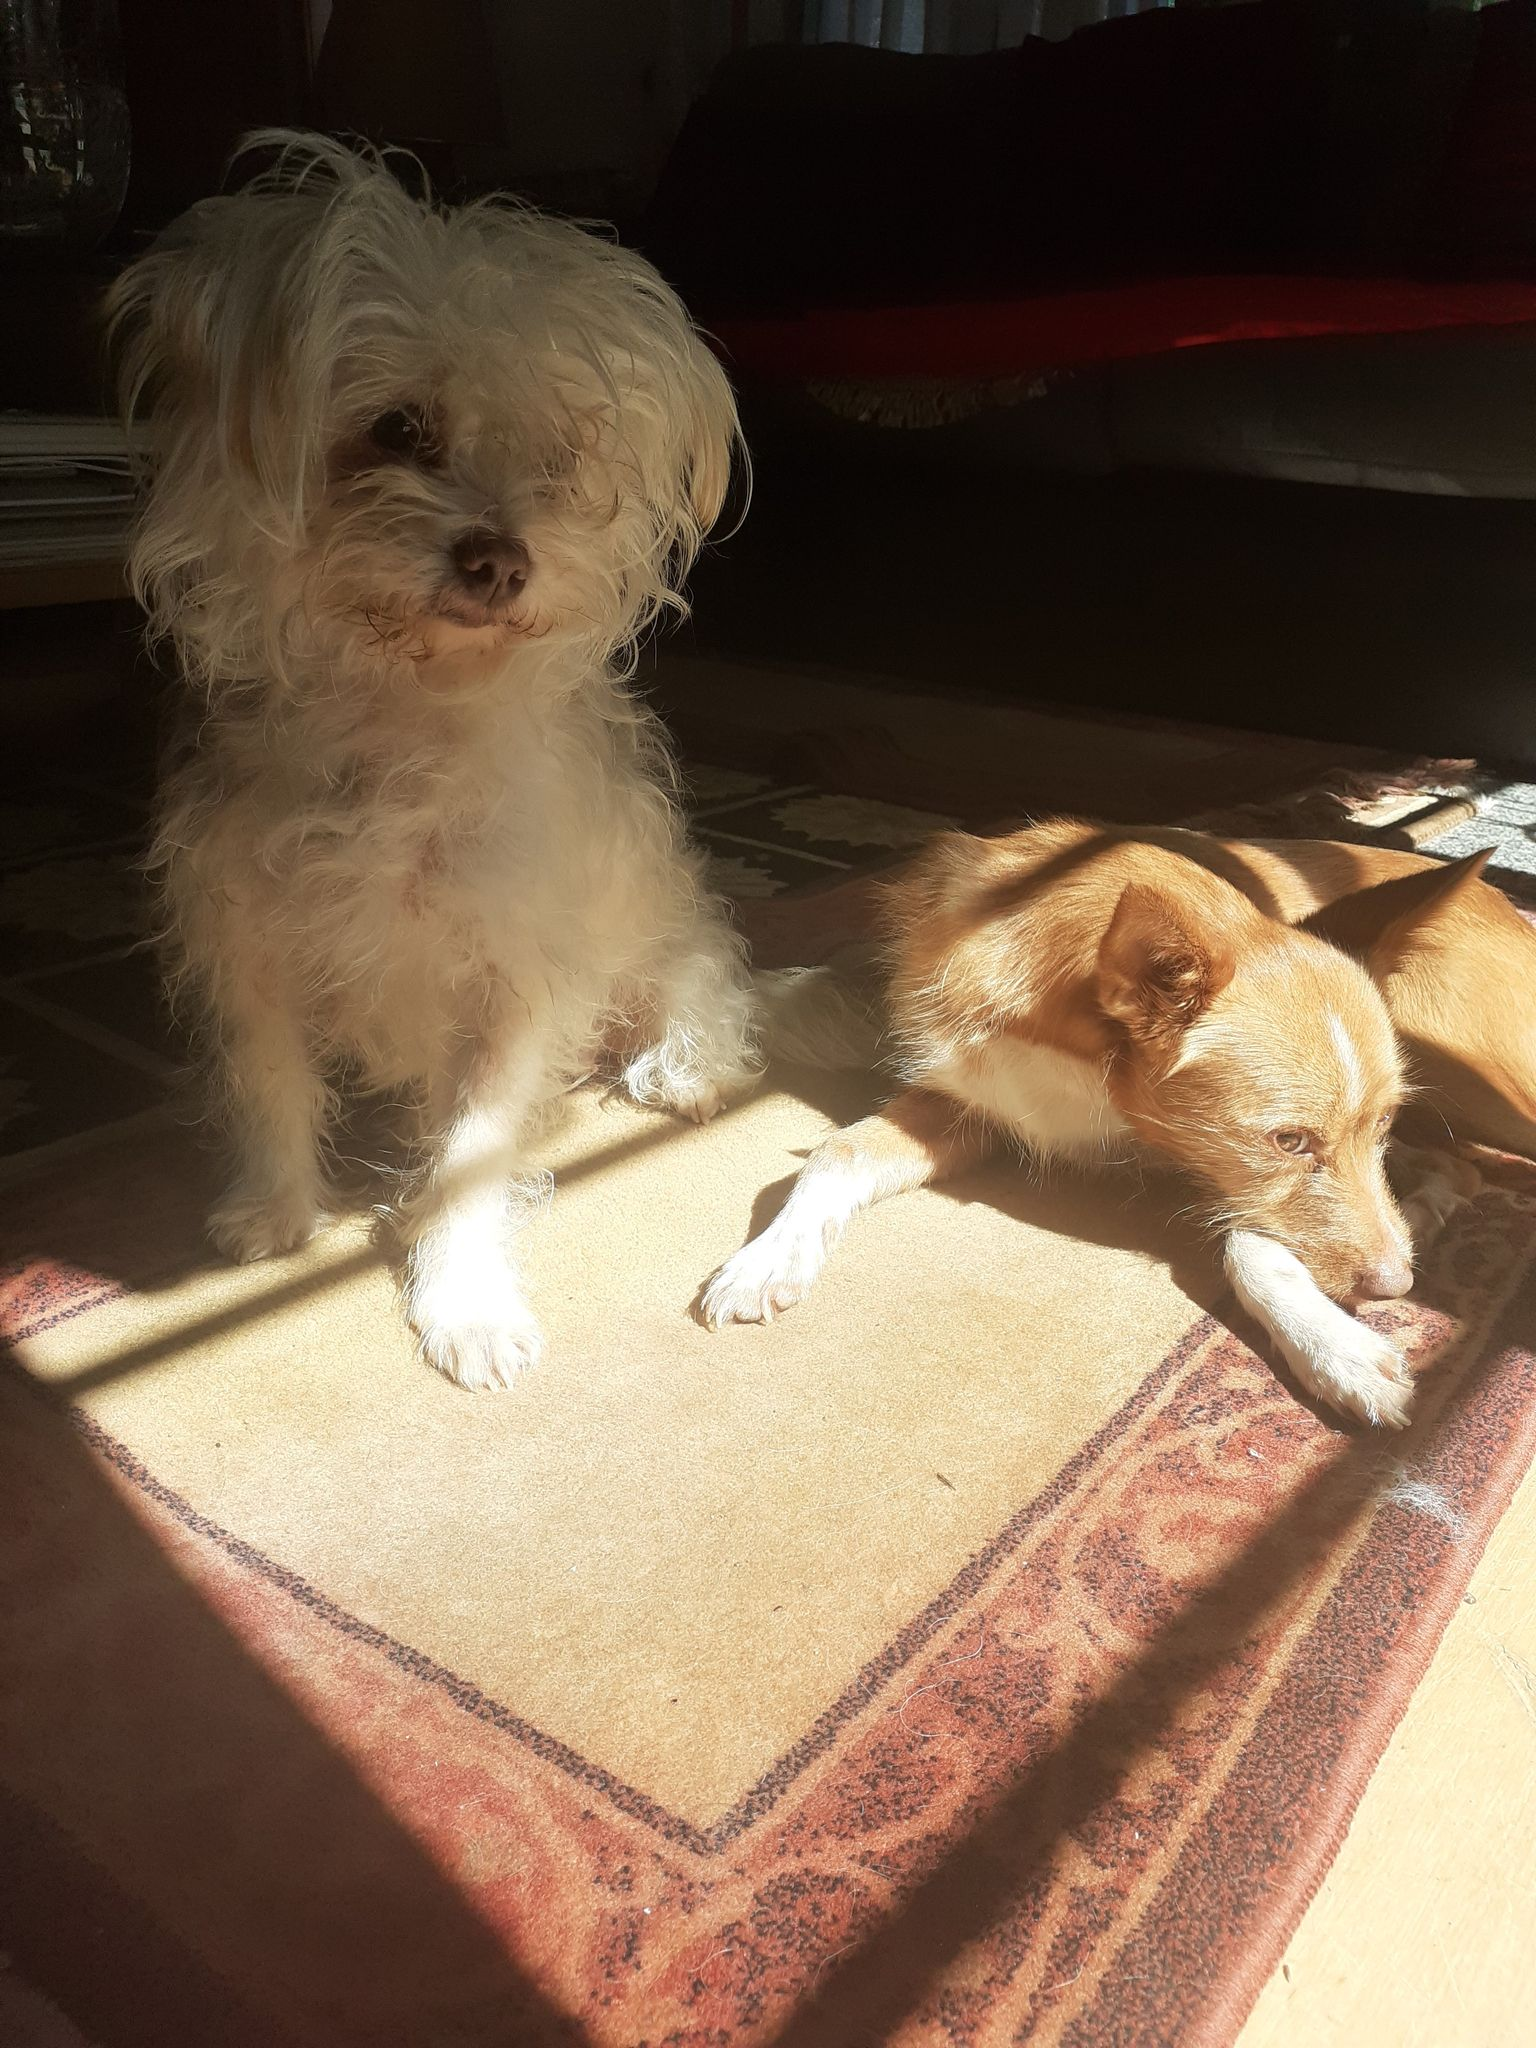
\includegraphics[width=\linewidth]{/mnt/c/Users/Duarte Vilar/OneDrive/Ambiente de Trabalho/Eu/tese/thesis/Thesis/Vilar/AdelinoVilar/ManuelVilar/ClaraVilar/DuarteVilar/p1-cadelas.jpg}
            \caption{a future caption here}
        \end{minipage}
        \hspace{1cm} % add some horizontal space here
        \begin{minipage}{0.3\textwidth}
            ok

            palavra 2

            palavra 3

            lasjgslakgjalkjgsalkj

            arroz
            
        \end{minipage}
    \end{figure}



    \begin{figure}[ht!]
        \begin{minipage}{0.35\textwidth}
            \centering
            \includegraphics[width=\linewidth]{/mnt/c/Users/Duarte Vilar/OneDrive/Ambiente de Trabalho/Eu/tese/thesis/Thesis/Vilar/AdelinoVilar/OUT/public/p1-Adelino.jpg}
            \caption{a future caption here}
        \end{minipage}
        \hspace{1cm} % add some horizontal space here
        \begin{minipage}{0.3\textwidth}
            ok

            palavra 2

            palavra 3

            lasjgslakgjalkjgsalkj

            arroz
            
        \end{minipage}
    \end{figure}



\newpage
\section{Meta-information}
\newcounter{tablecounter2}


    \stepcounter{tablecounter2}
    \begin{table}[ht!]
        \centering
        \begin{tabular}{|c|c|}
            \hline
            
                \textbf{ id } & \textit{ IndustriasReunidasvilar } \\
                \hline
            
                \textbf{ format } & \textit{ latex } \\
                \hline
            
                \textbf{ type } & \textit{ Story } \\
                \hline
            
                \textbf{ date } & \textit{ 1957-02-6 } \\
                \hline
            
        \end{tabular}
        \caption{A \textbf{ Story }-\textit{ IndustriasReunidasvilar }} % Add a caption to the table with the current table counter value
        \label{table:\arabic{tablecounter2}} % Use the current table counter value as the label name
    \end{table}

    \stepcounter{tablecounter2}
    \begin{table}[ht!]
        \centering
        \begin{tabular}{|c|c|}
            \hline
            
                \textbf{ id } & \textit{ IndustriasDeAdelinoVilar } \\
                \hline
            
                \textbf{ format } & \textit{ latex } \\
                \hline
            
                \textbf{ type } & \textit{ Story } \\
                \hline
            
                \textbf{ date } & \textit{ 19 de Março de 2017 } \\
                \hline
            
        \end{tabular}
        \caption{A \textbf{ Story }-\textit{ IndustriasDeAdelinoVilar }} % Add a caption to the table with the current table counter value
        \label{table:\arabic{tablecounter2}} % Use the current table counter value as the label name
    \end{table}

    \stepcounter{tablecounter2}
    \begin{table}[ht!]
        \centering
        \begin{tabular}{|c|c|}
            \hline
            
                \textbf{ id } & \textit{ EducaçãoPrimária } \\
                \hline
            
                \textbf{ format } & \textit{ latex } \\
                \hline
            
                \textbf{ type } & \textit{ Story } \\
                \hline
            
                \textbf{ date } & \textit{ 2022-09-15 } \\
                \hline
            
        \end{tabular}
        \caption{A \textbf{ Story }-\textit{ EducaçãoPrimária }} % Add a caption to the table with the current table counter value
        \label{table:\arabic{tablecounter2}} % Use the current table counter value as the label name
    \end{table}

    \stepcounter{tablecounter2}
    \begin{table}[ht!]
        \centering
        \begin{tabular}{|c|c|}
            \hline
            
                \textbf{ id } & \textit{ Pirolitos } \\
                \hline
            
                \textbf{ format } & \textit{ latex } \\
                \hline
            
                \textbf{ type } & \textit{ Story } \\
                \hline
            
                \textbf{ date } & \textit{ 2022-10-05 } \\
                \hline
            
        \end{tabular}
        \caption{A \textbf{ Story }-\textit{ Pirolitos }} % Add a caption to the table with the current table counter value
        \label{table:\arabic{tablecounter2}} % Use the current table counter value as the label name
    \end{table}

    \stepcounter{tablecounter2}
    \begin{table}[ht!]
        \centering
        \begin{tabular}{|c|c|}
            \hline
            
                \textbf{ id } & \textit{ viagemCaboVerde } \\
                \hline
            
                \textbf{ format } & \textit{ latex } \\
                \hline
            
                \textbf{ type } & \textit{ Story } \\
                \hline
            
                \textbf{ date } & \textit{ 2022 } \\
                \hline
            
        \end{tabular}
        \caption{A \textbf{ Story }-\textit{ viagemCaboVerde }} % Add a caption to the table with the current table counter value
        \label{table:\arabic{tablecounter2}} % Use the current table counter value as the label name
    \end{table}

    \stepcounter{tablecounter2}
    \begin{table}[ht!]
        \centering
        \begin{tabular}{|c|c|}
            \hline
            
                \textbf{ id } & \textit{ moto4 } \\
                \hline
            
                \textbf{ format } & \textit{ latex } \\
                \hline
            
                \textbf{ type } & \textit{ Story } \\
                \hline
            
                \textbf{ date } & \textit{ 2022 } \\
                \hline
            
        \end{tabular}
        \caption{A \textbf{ Story }-\textit{ moto4 }} % Add a caption to the table with the current table counter value
        \label{table:\arabic{tablecounter2}} % Use the current table counter value as the label name
    \end{table}

    \stepcounter{tablecounter2}
    \begin{table}[ht!]
        \centering
        \begin{tabular}{|c|c|}
            \hline
            
                \textbf{ id } & \textit{ RoupaASecar } \\
                \hline
            
                \textbf{ format } & \textit{ latex } \\
                \hline
            
                \textbf{ type } & \textit{ Story } \\
                \hline
            
                \textbf{ date } & \textit{ 2023-01-7 } \\
                \hline
            
        \end{tabular}
        \caption{A \textbf{ Story }-\textit{ RoupaASecar }} % Add a caption to the table with the current table counter value
        \label{table:\arabic{tablecounter2}} % Use the current table counter value as the label name
    \end{table}

    \stepcounter{tablecounter2}
    \begin{table}[ht!]
        \centering
        \begin{tabular}{|c|c|}
            \hline
            
                \textbf{ id } & \textit{ Pobreza } \\
                \hline
            
                \textbf{ format } & \textit{ latex } \\
                \hline
            
                \textbf{ type } & \textit{ Story } \\
                \hline
            
                \textbf{ date } & \textit{ 2023-01-12 } \\
                \hline
            
        \end{tabular}
        \caption{A \textbf{ Story }-\textit{ Pobreza }} % Add a caption to the table with the current table counter value
        \label{table:\arabic{tablecounter2}} % Use the current table counter value as the label name
    \end{table}


\end{document}
